%\subtask{Describe and discuss your ``objective method'', ie. the method by which you will measure the success of your predictor.}

The functionality of the system will be verified by doing regular predictions and comparing these to the actual 
parking situation later. Similar to the crawling implementation, the web application will generate a new prediction 
``15 minutes into the future''. These predictions will be saved in a database. 

To measure the error, we will use the mean absolute error 
\[
MAE \defeq mean(|y_i^∗ − y_i|)\text{.}
\]

The evaluations were fetched on 2017-03-11 at 6pm. Tables \ref{tab:eval_doy} and \ref{tab:eval_woy} list the \(MAE\)

\begin{table}
  \centering
  \caption{Evaluation per day of year}
  \label{tab:eval_doy}
  \begin{tabular}{rrrr}
  \(date\) & \(n\) & \(MAE\) & \(\sigma\) \\
  \hline 
  01.03.   &  103  &   26.14 &  36.35 \\
  02.03.   &  185  &   23.64 &  29.54 \\
  03.03.   &  286  &   21.24 &  24.80 \\
  04.03.   &  521  &   39.06 &  36.61 \\
  05.03.   & 1091  &   67.32 &  47.67 \\
  06.03.   & 1082  &   51.28 &  45.73 \\
  07.03.   &  925  &  204.89 & 127.97 \\
  08.03.   &  969  &  186.90 & 172.56 \\
  09.03.   & 1050  &   20.70 &  28.86 \\
  10.03.   & 1085  &   25.24 &  27.12 \\
  11.03.   &  586  &   30.31 &  40.46 \\
  \end{tabular}
\end{table}

\begin{table}
  \centering
  \caption{Evaluation per week of year}
  \label{tab:eval_woy}
  \begin{tabular}{rrrr}
  \(\woy\) & \(n\) & \(MAE\) & \(\sigma\) \\
  \hline 
   8       &  640  & 23.12   &  30.50 \\
   9       & 6723  & 84.64   & 112.68 \\
  10       &  618  & 30.49   &  39.62 \\
  \hline
  \end{tabular}
\end{table}

\begin{figure}
  \centering
  \caption{Crawled parking space availability}
  \label{fig:actual}
  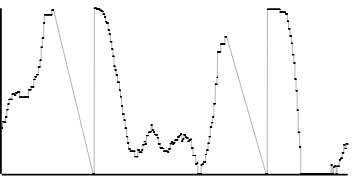
\includegraphics[scale=0.5]{fig_actual}
\end{figure}

\begin{figure}
  \centering
  \caption{Predicted parking space availability}
  \label{fig:predictions}
  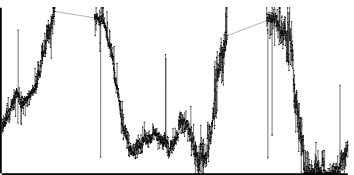
\includegraphics[scale=0.5]{fig_predictions}
\end{figure}


TODO\todo{what do these numbers mean?}\todo{how did we achieve them?}

\todo{how do we verify?}
\todo{what method do we use to measure error?}
\todo{verification over time?}
\todo{implementation}

At the moment, the predictions are of very bad quality and not usable. For 403 predictions, the average absolute error had a mean of \(144.14\) with a standard deviation of \(99.68\).

In rare cases, the predictions are quite good. \(47\) predictions were off by less than \(20\), 
\(19\) predictions were off by less than \(10\), and \(6\) predictions were off by less than 2. One goal -- beside improving the prediction accuracy overall -- will be to understand why these predictions were so good.

The original predictions were achieved by training a RegressionTree on tuples of the form 
\[
((\hod, \moh, \dow, \dom, \wom, \woy, \yyy), free)\text{.}
\]
Since these results are very unsatisfactory, other methods will be investigated until the final report.